% Term paper — Advanced Topics in Computational Text and Media Sciences #1, SoSe 2026
% Universität Trier — Group I, World Knowledge I
% Uses the official preprint template (arxiv.sty), unaltered.
% Compile: pdflatex negation_paper.tex (twice)
% Code, data and outputs: https://github.com/PriyadithGowda/negprobe
\documentclass{article}

\usepackage{arxiv}

\usepackage[utf8]{inputenc}
\usepackage[T1]{fontenc}
\usepackage[numbers,round]{natbib}
\usepackage{hyperref}
\usepackage{url}
\usepackage{booktabs}
\usepackage{amsfonts}
\usepackage{amsmath}
\usepackage{nicefrac}
\usepackage{microtype}
\usepackage{graphicx}
\usepackage{xcolor}

\title{Birds Can Still Not Fly? Negation in Factual Probes from BERT to Modern Language Models}

\author{
  Priyadith Hosahalli Nagesh \\
  Universität Trier \\
  Advanced Topics in Computational Text and Media Sciences \#1 \\
  \texttt{s2prhosa@uni-trier.de} \\
}

\renewcommand{\shorttitle}{Negation in Factual Probes}
\hypersetup{
pdftitle={Negation in Factual Probes from BERT to Modern Language Models},
pdfauthor={Priyadith Hosahalli Nagesh},
pdfkeywords={negation, probing, language models, LAMA, knowledge},
colorlinks=true, linkcolor=black, citecolor=black, urlcolor=black,
}

\begin{document}
\maketitle

\begin{abstract}
\citet{kassner2020} showed that pretrained language models barely distinguish a cloze query from its negation: BERT-large completes both ``Birds can [MASK]'' and ``Birds cannot [MASK]'' with \emph{fly}. We replicate that result and extend it along three axes. First, we introduce a
probability-based measure of negation sensitivity, the change $\Delta$ in the log probability the
model assigns to the denied fact, and show that it can rank models differently from the original rank-based metrics. Second, we compare masked and autoregressive models on an identical set of probes. Third, we test whether the failure survives a change of probe format by
having a base and an instruction-tuned model judge negated statements as true or false. The replication succeeds:
on T-REx, BERT-base returns the same top-ranked answer for the affirmative and the negated query in
51.9\,\% of cases with the released templates and 54.1\,\% with corrected ones (34{,}039 pairs, averaged over relations). The extensions qualify the original conclusion. An instruction-tuned model
with 1.5B parameters judges negated statements correctly in 62.2\,\% of cases against 50\,\% chance: it does register the negation, but the gap in its rate of ``True'' answers between true and false statements shrinks from 55 points for affirmative to 24 points for negated statements, and a strong bias towards answering ``False'' makes its accuracy uneven (0.911 on false negated statements, 0.332 on true ones). Its base model knows the facts about as well but barely registers the negation (a 5-point gap, 52.5\,\% correct). The cloze probe overstates the failure; the truth-judgement probe measures it more precisely, provided it is read cell by cell. In the course of the replication we also
identified an off-by-one error in the released relation templates that assigns the wrong negated
template to two of the 41 T-REx relations and measurably distorts aggregate results.
\end{abstract}

\keywords{negation \and probing \and language models \and factual knowledge \and LAMA}

\section{Introduction}
\label{sec:intro}

The claim that pretrained language models store factual knowledge rests largely on cloze probes. A
model is shown a sentence with a gap, ``Dante was born in \underline{\hspace{1em}}'', and is scored on
whether the filler it ranks first is the right entity \citep{petroni2019}. Success on such probes has
been read as evidence that the model contains a knowledge base of sorts, retrievable by natural
language query.

Negation puts that reading under stress. A model that understands ``$X$ was \emph{not} born in
\underline{\hspace{1em}}'' should treat it very differently from the affirmative sentence: the one
filler that is certainly wrong is the true birthplace. \citet{kassner2020} constructed exactly this
contrast for the LAMA probes and found that pretrained models fail it. Their title names two failures: primed with ``Talk?'', BERT-large completes ``Birds can [MASK]'' with \emph{talk}, and it completes the negated ``Birds cannot [MASK]'' with \emph{fly}.

What that failure means is not settled. Three readings compete. On the first, the models are simply
insensitive to negation, a deficit that both \citet{truong2023} and \citet{garciaferrero2023} trace to the pretraining objective and that larger models do not remove. On the second, the deficit is representational and fixable with
a different training signal, as \citet{hosseini2021} show by training with an unlikelihood objective.
On the third, the negated cloze probe is a peculiar task --- the negated query has no unique correct
answer, so a model that keeps its prediction is not straightforwardly wrong --- and the measured
failure is partly an artefact of the instrument.

This paper is designed to separate the third reading from the first two. We ask:

\begin{description}
  \item[RQ1] Do the negated-LAMA results of \citet{kassner2020} replicate under a re-implementation?
  \item[RQ2] Does negation sensitivity change with scale within a controlled model family?
  \item[RQ3] Do masked and autoregressive models differ when probed on identical items?
  \item[RQ4] Does the failure persist when the same facts are probed by truth judgement instead?
\end{description}

\paragraph{Contributions.}
\begin{enumerate}
  \item A replication of the negated LAMA experiment for BERT-base and BERT-large on all 39{,}567
  Google-RE and T-REx pairs (Section~\ref{sec:results-rep}).
  \item $\Delta$, a probability-based measure of negation sensitivity that remains defined when the
  negated query has no unique answer, and which can rank models differently from overlap
  (Sections~\ref{sec:method} and~\ref{sec:results-delta}).
  \item A like-for-like comparison of a masked and an autoregressive model on an identical subset of
  probes (Section~\ref{sec:results-arch}).
  \item Evidence from a balanced truth-judgement probe that an instruction-tuned model registers negation, though less reliably than affirmation and under a strong bias towards answering ``False'', while its base model barely does (Section~\ref{sec:results-truth}).
  \item The identification and correction of an off-by-one error in the released relation templates
  (Section~\ref{sec:data-error}).
\end{enumerate}

Code and configurations are available at \url{https://github.com/PriyadithGowda/negprobe}.%
\footnote{Citations use a numbered system (bracketed numbers, with author names where they are
named in the text); the bibliography is ordered alphabetically and formatted consistently, and every entry gives a DOI, an arXiv identifier or a public URL. The paper is written in
English and uses ``we'' in the conventional sense of the author's voice; it contains no references to
persons that would require a gender-inclusive strategy.}

\section{Background}
\label{sec:background}

\paragraph{The LAMA probe.} The probe spans four sources: Google-RE, T-REx, ConceptNet and SQuAD \citep{petroni2019}. For Google-RE and T-REx, cloze statements are built from knowledge-base triples: each relation carries a template --- ``[X] was born in [Y] .'' for \textit{place of birth} --- which is instantiated with a subject and masked at the object position; ConceptNet uses masked sentences from the Open Mind Common Sense corpus and SQuAD manually rewritten questions. Models are ranked over a shared vocabulary and scored with precision at one (P@1).

\paragraph{Negated LAMA.} \citet{kassner2020} negate every LAMA template or question (for ConceptNet, an easy-to-negate subset) and compare the predictions for original and negated queries using the Spearman rank correlation and the share of pairs whose top-ranked filler is identical. For all five models they test (Transformer-XL, two ELMo variants, BERT-base and BERT-large) the rank correlation is above 85\,\% in most cases. In a controlled synthetic experiment, BERT pretrained on affirmative and negated sentences fails to generalise to held-out facts, whereas BERT fine-tuned to classify the sentences as true or false succeeds; they conclude that BERT ``easily learns negation if supervision is available, but fails without it''.

\paragraph{Competence and performance.} The distinction between competence and performance is directly at stake. A system may deliver correct factual answers yet fail to process negation, thereby displaying performance without the corresponding competence; the psycholinguistic diagnostics of \citet{ettinger2020} are one way of testing for this, as controlled word-prediction tests that ask what information a model uses when predicting in context. RQ4 emphasises this issue: when a model succeeds with one probe design but fails with another, the benchmark is partly measuring the format itself.

\section{Related Work}
\label{sec:related}

\paragraph{Negation in pretrained models.} \citet{ettinger2020} finds BERT's predictions largely
unaffected by negation in a psycholinguistic setting, independently of LAMA. \citet{hosseini2021}
further train BERT with an unlikelihood objective on automatically negated generic sentences from Wikipedia, reducing top-1 error on negated LAMA to 4\,\% while keeping scores on the original LAMA queries and on natural language inference roughly unchanged.

\paragraph{Does scale help?} \citet{truong2023} evaluate GPT-neo, OPT, GPT-3, InstructGPT and FLAN-T5 at several
sizes across negation benchmarks and find that larger models are, if anything, more insensitive to negation, with instruction tuning helping more than scale; they
distinguish insensitivity to the presence of negation, failure to capture its lexical semantics, and
failure to reason under it. \citet{garciaferrero2023} introduce a benchmark of roughly 400{,}000
sentences and find that models classify affirmative sentences well while relying on superficial cues
for negated ones, with fine-tuning failing to generalise. \citet{mckenzie2023} document tasks on which
larger models perform worse, showing that scale is not monotonically beneficial.

\paragraph{Positivity bias.} \citet{chen2023} show that large models generate sentences grounded in negative commonsense knowledge much less reliably than in positive knowledge, even when they answer the corresponding yes-or-no questions correctly. Our
truth-judgement experiment measures a closely related quantity directly, the rate at which a model
answers ``True'' on a balanced item set (Section~\ref{sec:results-truth}).

\paragraph{Positioning.} Prior work either replicates the cloze finding on newer models or builds new
benchmarks. To our knowledge no study applies the \emph{original} negated LAMA probes to a controlled
scaling suite, to masked and autoregressive models on a matched item set, and to a second probe format while holding templates and metrics fixed,
so that differences are attributable to models rather than to benchmarks. That is the gap addressed
here.

\section{Data and Models}
\label{sec:data}

\paragraph{Probes.} We use the negated LAMA release accompanying \citet{kassner2020}. Negated
templates for T-REx are provided in \texttt{relations.jsonl}; SQuAD samples and the negated subset of ConceptNet samples carry a
\texttt{negated} field; Google-RE has neither, and its templates are those hard-coded in the LAMA
evaluation scripts. For Google-RE and T-REx we generate both the affirmative and the negated sentence
from the relation templates, so that the two differ only in the negation. This paper uses Google-RE
(3 relations, 5{,}528 pairs) and T-REx \citep{elsahar2018} (41 relations, 34{,}039 pairs); ConceptNet and SQuAD are left
for future work because their negations are sample-specific rather than template-generated.

\paragraph{Models.} BERT-base-cased and BERT-large-cased \citep{devlin2019}, with 110M and 340M parameters, represent masked language models.
Pythia-410m \citep{biderman2023} represents autoregressive models; its family holds training data and
ordering fixed across sizes, which makes it the appropriate suite for a scaling claim. For truth
judgement we use Qwen2.5-1.5B-Instruct \citep{qwen2025} and the base model it was post-trained from, Qwen2.5-1.5B.
We evaluate Pythia at 410m and 1.4b parameters; the larger members of the suite
were not reachable within the compute available (Section~\ref{sec:limitations}).

\paragraph{Adapting the probes to autoregressive models.} An autoregressive model predicts only the
continuation of a prefix, so only pairs whose mask is the final content token are usable. This retains
28{,}764 of 34{,}039 T-REx pairs (84.5\,\%) and all Google-RE pairs. For a like-for-like comparison we
restrict BERT's outputs to exactly that subset (Section~\ref{sec:results-arch}). Candidates are ranked over the
LAMA common vocabulary, restricted per model to entries that are a single token under its own
tokenizer, giving 21{,}018 entries for BERT and 15{,}800 for Pythia; we report both, since a smaller
candidate set makes the task easier.

\section{Method}
\label{sec:method}

\paragraph{Experiment A: replication metrics.} For each pair we compute the Spearman rank correlation
$\rho$ between the affirmative and negated distributions over the restricted vocabulary, and whether
the top-ranked filler is identical (\emph{overlap}). P@1 is the share of pairs whose top-ranked candidate is the gold object itself; for an autoregressive model this requires the gold object to be a single token in its candidate set. Following \citet{petroni2019} we compute scores per relation and then average across relations; micro averages over all pairs can differ noticeably (by up to 0.05 in overlap and 0.27 in $\Delta$ on Google-RE), so both are given in the repository and compared for T-REx in the appendix.

\paragraph{Experiment B: the negation shift.} The rank-based metrics are indirect. Under negation
nearly any filler except the gold object is defensible, so a changed top prediction is not by itself
evidence of understanding, and an unchanged one is not proof of failure. To assess this, we calculate the difference in log probability assigned to the denied fact,
\begin{equation}
\Delta = \log P(o_{\text{gold}} \mid s_{\text{neg}}) - \log P(o_{\text{gold}} \mid s_{\text{aff}}),
\label{eq:delta}
\end{equation}
where $s_{\text{aff}}$ and $s_{\text{neg}}$ are identical except for the presence of negation. If a model truly recognises negation, $\Delta$ should drop well below zero. For masked models, as in LAMA, the gold object must be a single token; for autoregressive models, $\Delta$ aggregates the log probabilities across all tokens of the gold object.

\paragraph{Experiment C: truth judgement.} Every fact is tested using four statements arranged in a $2 \times 2$ format, combining both affirmation and negation with either the gold object or a distractor drawn from the same relation. For the gold object, the affirmative statement is true and the negated one false; for the distractor, the truth values are reversed. Instead of relying on generated text, verdicts are determined by the probabilities assigned to the \emph{True} and \emph{False} tokens, which makes results deterministic and eliminates parsing. Instruction-tuned models are prompted through their chat template; a base model receives four fixed examples instead (\texttt{--chat no}, since Qwen2.5 base models also ship a chat template). The reported metrics are accuracy by polarity, the \emph{negation gap} (the difference between the two), \emph{pair consistency} (the share of statement pairs --- one fact with one object --- whose verdict flips between the affirmative and the negated statement), accuracy on negated items restricted to facts whose affirmative statement is judged correctly (isolating negation errors from lack of knowledge), and the overall frequency of ``True'' responses.

\paragraph{Experiment D: free generation.} In this experiment, the model is prompted to complete a sentence containing a negation; giving the denied fact is treated as a mistake, while the affirmative completion serves as a control for knowledge. Although this method is available in the published code, it was not executed because of the computational constraints of this study, and no findings from it are presented.

\paragraph{Implementation note.} All experiments are implemented in Python with PyTorch
\citep{paszke2019} and the Hugging Face Transformers library \citep{wolf2020}, which also supplies
every model checkpoint. One detail had a significant impact. Half precision without a CUDA device produced non-finite values in our runs (float16 on CPU for Pythia, bfloat16 on an Apple M1), leading to rankings that falsely appear perfectly accurate. This issue affected our initial Pythia run. The code has since been updated to terminate if any score is non-finite and to default to full precision when no CUDA device is present. All reported runs use float32: BERT on an Apple M1 CPU, Pythia and Qwen on a Colab T4 GPU.  We highlight this because it is a silent failure that could easily go undetected and be published.

\section{Results}
\label{sec:results}

\subsection{RQ1: the replication holds}
\label{sec:results-rep}

Table~\ref{tab:main} reports Experiments A and B. With the templates as released --- the
configuration distributed with \citet{kassner2020} --- BERT-base returns the same top-ranked filler for the affirmative and the negated query in, on average over relations, 51.9\,\% of T-REx pairs, with mean rank correlation 0.866;
BERT-large behaves similarly (46.9\,\%, $\rho = 0.832$). With the templates corrected
(Section~\ref{sec:data-error}) the figures are 54.1\,\% and 49.1\,\%. Either way this reproduces the
qualitative finding of \citet{kassner2020}. Typical cases leave little room for interpretation:

\begin{quote}\small
\texttt{President of Mexico is a legal term in [MASK] . $\rightarrow$ Mexico}\\
\texttt{President of Mexico is not a legal term in [MASK] . $\rightarrow$ Mexico}
\end{quote}

\begin{table}[t]
\centering\small
\caption{Experiments A and B. $\rho$ and overlap compare the affirmative and negated distributions;
$\Delta$ is the change in the log probability of the gold object (Eq.~\ref{eq:delta}). Averages are
taken within a relation, then across relations. ``As released'' uses \texttt{relations.jsonl}
unchanged; ``repaired'' corrects the two wrong negated templates and keeps all 41 relations
(Section~\ref{sec:data-error}).}
\label{tab:main}
\begin{tabular}{llrrrrrr}
\toprule
Model & Data & $N$ & $\rho$ & Overlap & $\Delta$ & P@1 & P@1 (neg.) \\
\midrule
BERT-base   & Google-RE & 5{,}528  & 0.834 & 0.113 & $-0.814$ & 0.099 & 0.028 \\
BERT-large  & Google-RE & 5{,}528  & 0.776 & 0.112 & $-0.840$ & 0.105 & 0.028 \\
Pythia-410m & Google-RE & 5{,}528  & 0.881 & 0.259 & $-0.748$ & 0.045 & 0.013 \\
\midrule
BERT-base   & T-REx (as released) & 34{,}039 & 0.866 & 0.519 & $-0.735$ & 0.311 & 0.237 \\
BERT-large  & T-REx (as released) & 34{,}039 & 0.832 & 0.469 & $-1.018$ & 0.323 & 0.251 \\
BERT-base   & T-REx (repaired)    & 34{,}039 & 0.887 & 0.541 & $-0.568$ & 0.311 & 0.237 \\
BERT-large  & T-REx (repaired)    & 34{,}039 & 0.852 & 0.491 & $-0.840$ & 0.323 & 0.251 \\
\bottomrule
\end{tabular}
\end{table}

\begin{figure}[t]
\centering
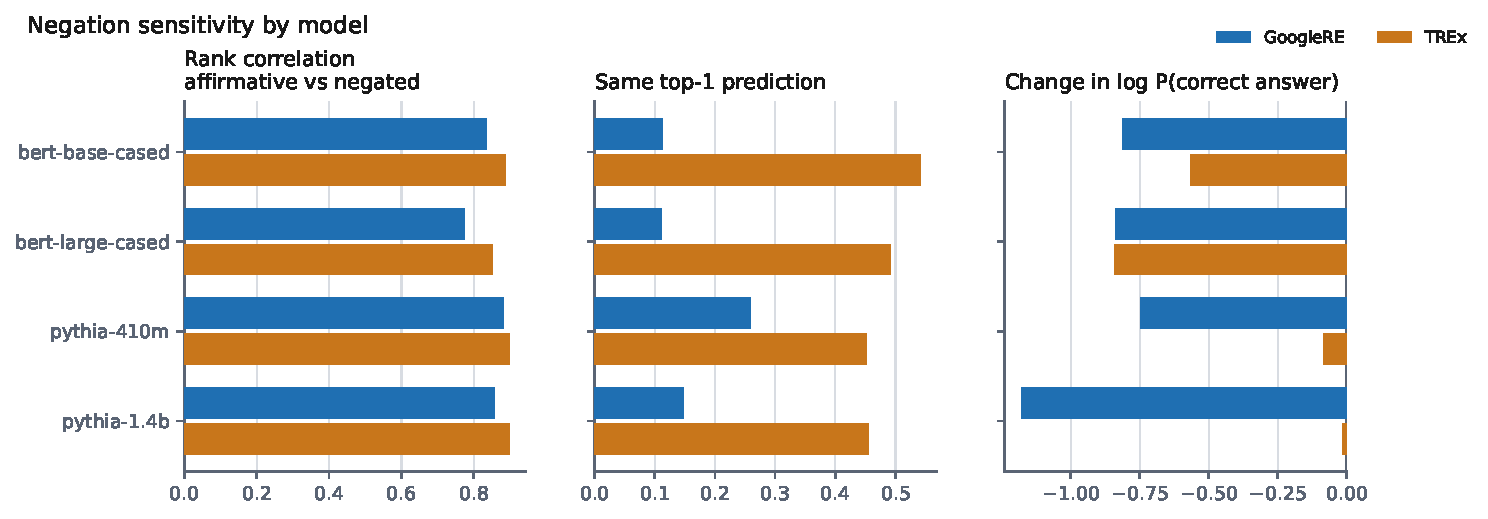
\includegraphics[width=\textwidth]{fig1_model_comparison.pdf}
\caption{Negation sensitivity by model and subset. Rank correlation and overlap (left, centre) are the
metrics of \citet{kassner2020}; the change in the log probability of the denied fact (right) is
introduced here. BERT bars use all pairs, Pythia bars the mask-final pairs an autoregressive model can score, so cross-model comparisons should rest on Table~\ref{tab:common}.}
\label{fig:models}
\end{figure}

\subsection{RQ1b: $\Delta$ and overlap measure different things}
\label{sec:results-delta}

Scale within the BERT family barely moves the rank-based metrics: with repaired templates, overlap
falls from 0.541 to 0.491 between base and large, five points. $\Delta$ moves much more in relative
terms, from $-0.568$ to $-0.840$ (macro averages); over all pairs the means are $-0.590$ and $-0.906$, with disjoint 95\,\% bootstrap intervals $[-0.606, -0.573]$ and $[-0.934, -0.879]$. Much of this difference is concentrated in a few relations: for P36 (\textit{capital}) BERT-large's $\Delta$ is $-9.98$ against $-3.35$ for BERT-base, and without P36 the macro averages are $-0.498$ and $-0.611$; the median pair barely differs ($-0.199$ against $-0.185$). The larger model therefore pushes the denied fact much further down on some relations, while its top answer changes only somewhat more often; overlap and $\Delta$ rank the two models the same way but weigh them very differently. The same contrast holds on the released
templates ($-0.735$ vs.\ $-1.018$), so it does not depend on the repair.

Across the 41 T-REx relations the two measures correlate at $r = 0.578$: they agree in direction and
diverge in detail (Figure~\ref{fig:relations}). Negation sensitivity is strongly relation-dependent.
For BERT-base, overlap reaches 0.947 for P463 (\textit{member of}) and 0.915 for P1376
(\textit{capital of}), and falls to 0.000 for P103 (\textit{native language}) and 0.013 for P364
(\textit{original language of work}), where $\Delta$ is $-4.73$ and $-4.35$. P103 is instructive: the
model answers the affirmative query correctly 72.2\,\% of the time and the negated one 0.0\,\% of the
time, which is how a competent negation handler would behave. Negation failure is therefore not
uniform across the probe, and a single aggregate hides relations at both extremes. Within Google-RE, overlap is 0.011 for birth dates, 0.112 for birth
places and 0.217 for places of death: a fine-grained numeric answer space behaves unlike an entity
answer space, which argues against reporting one figure per model.

\begin{figure}[t]
\centering
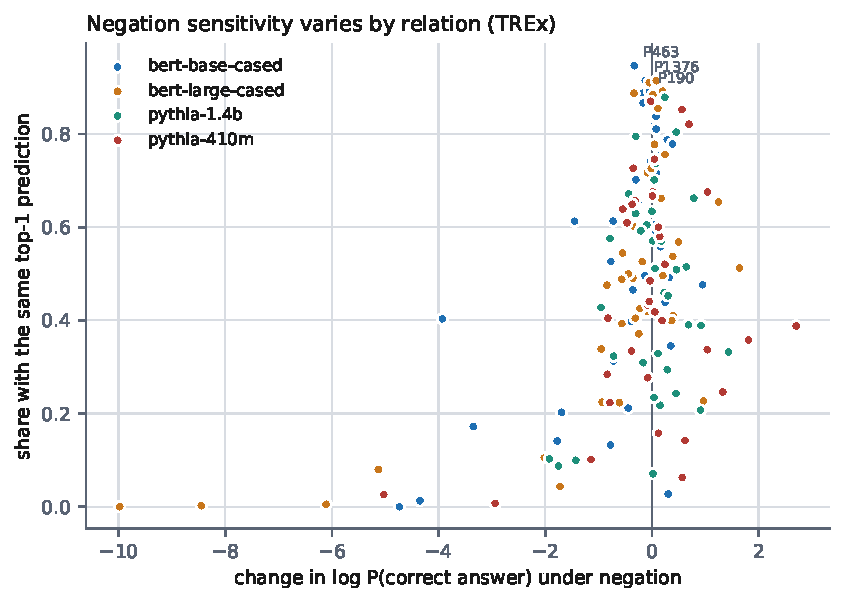
\includegraphics[width=0.72\textwidth]{fig3_per_relation.pdf}
\caption{Per-relation means on T-REx. Relations cluster near zero change in the denied fact's
probability while a tail suppresses it strongly; all four models show the same shape. Pythia points cover the 35 relations with mask-final pairs. The leftmost point is BERT-large on P36.}
\label{fig:relations}
\end{figure}

\subsection{An error in the released templates}
\label{sec:data-error}

The file \texttt{relations.jsonl} of the negated LAMA release assigns the wrong negated template to two
relations: P103 (\textit{native language}) receives the negation belonging to P127
(\textit{owned by}), and P190 (\textit{twinned administrative body}) receives the one belonging to
P103. For those relations the ``negated'' sentence is an unrelated statement:

\begin{quote}\small
\texttt{The native language of [X] is [Y] .}\hfill(affirmative, P103)\\
\texttt{[X] is not owned by [Y] .}\hfill(``negated'', as released)
\end{quote}

The consequence is not cosmetic. As released, these two relations show the largest negation effects in
the entire probe --- overlap 0.000 with $\Delta$ of $-6.54$ and $-5.10$ for BERT-base --- because the
model is being asked to complete a different sentence, not a negated one. Repairing the templates moves
the aggregate $\Delta$ from $-0.735$ to $-0.568$ for BERT-base and from $-1.018$ to $-0.840$ for
BERT-large, and raises overlap by about two points; roughly a fifth of the measured negation effect in
the released configuration was an artefact of two relations out of 41.

The two relations behave very differently once repaired, which is itself informative. P190 becomes one
of the least negation-sensitive relations in the probe (overlap 0.892, $\Delta = -0.04$): the model
ignores \emph{not} in ``[X] and [Y] are not twin cities'' almost entirely. P103 remains an extreme case
in the other direction (overlap 0.000, $\Delta = -4.73$), so its apparent sensitivity was not purely an
artefact. To clearly differentiate these scenarios, we treat the results from the corrected configuration as the main version in our report.

We update the templates to ``The native language of [X] is not [Y] .'' and ``[X] and [Y] are not twin cities .'', with our code systematically comparing each negated template to its corresponding affirmative and issuing a warning if there is any discrepancy. Before the correction, the check flags exactly these two relations, and none afterwards. Given the popularity of this release, the error may have affected results reported in other studies, though we have not conducted a comprehensive review of that literature.

\subsection{A common item set for cross-model comparison}
\label{sec:common}

Since models vary in which items they can score, Table~\ref{tab:common} restricts all models to a shared item set: the 28{,}764 mask-final T-REx pairs, spanning 35 relations (P190 drops out because its repaired template does not end in the object). Every row is computed on identical items with repaired templates, so the comparison is exact rather than approximate.

\begin{table}[t]
\centering\small
\caption{Identical 28{,}764 mask-final T-REx pairs (35 relations) for all four models, repaired templates.}
\label{tab:common}
\begin{tabular}{lrrrrr}
\toprule
Model & $\rho$ & Overlap & $\Delta$ & P@1 & P@1 (neg.) \\
\midrule
BERT-base   & 0.880 & 0.517 & $-0.491$ & 0.363 & 0.277 \\
BERT-large  & 0.842 & 0.487 & $-0.817$ & 0.376 & 0.292 \\
Pythia-410m & 0.900 & 0.452 & $-0.083$ & 0.226 & 0.221 \\
Pythia-1.4b & 0.899 & 0.455 & $-0.016$ & 0.239 & 0.231 \\
\bottomrule
\end{tabular}
\end{table}

\subsection{RQ3: masked versus autoregressive models}
\label{sec:results-arch}

On the common item set of Section~\ref{sec:common} (Table~\ref{tab:common}), Pythia-410m changes its
top prediction more often than BERT-base (overlap 0.452 vs.\ 0.517) yet lowers the gold object far less
($\Delta = -0.083$ vs.\ $-0.491$), and its accuracy is essentially unaffected by the negation
($0.226 \rightarrow 0.221$, against $0.363 \rightarrow 0.277$ for BERT-base). Although the autoregressive model adjusts its predictions, it does not suppress the denied fact. If only overlap were considered, Pythia would appear more sensitive to negation; however, $\Delta$ reverses this outcome, and the P@1 values support the assessment of $\Delta$. The same holds against BERT-large, the masked model closest in size to Pythia-410m (340M parameters, against 302M non-embedding parameters for Pythia-410m): overlap 0.487, $\Delta = -0.817$, P@1 $0.376 \rightarrow 0.292$.


\subsection{RQ2: scale does not buy negation sensitivity}
\label{sec:results-scale}

Within each family, more parameters bring more factual knowledge. BERT-base to BERT-large raises P@1
from 0.363 to 0.376; Pythia-410m to Pythia-1.4b raises it from 0.226 to 0.239. Negation sensitivity does
not follow.

For the Pythia pair there is no improvement. $\Delta$ is close to zero at both sizes ($-0.083$ and $-0.016$; $+0.001$ and $+0.026$ without P36), and the accuracy gap between affirmative and negated queries is small at both sizes (0.226 against 0.221, and 0.239 against 0.231), so adding \emph{not} to the sentence leaves the success rate unchanged. The model that knows more facts does not suppress the denied fact more.

The BERT pair does move: BERT-large suppresses the denied fact more ($\Delta$ from $-0.491$ to $-0.817$, or from $-0.407$ to $-0.548$ without P36), so the two families do not behave alike. Figure~\ref{fig:scaling} also shows that the direction differs even within a family: on Google-RE, Pythia's $\Delta$ deepens with scale ($-0.748$ to $-1.180$) while on T-REx it
flattens. Google-RE consists of three biographical relations with answer spaces (dates, cities) quite
unlike T-REx's, and this is exactly where the per-relation variation of
Section~\ref{sec:results-delta} reappears at the level of subsets.

The safe conclusion is the negative one, and it agrees with \citet{truong2023} from a different
direction: across the range we can test, no consistent improvement in negation handling accompanies scale: it appears in one family, is absent in the other, and in the BERT family rests largely on a few relations. Two model families and two
sizes each cannot establish a scaling law; they are sufficient to show that improvement is not
automatic.

\begin{figure}[t]
\centering
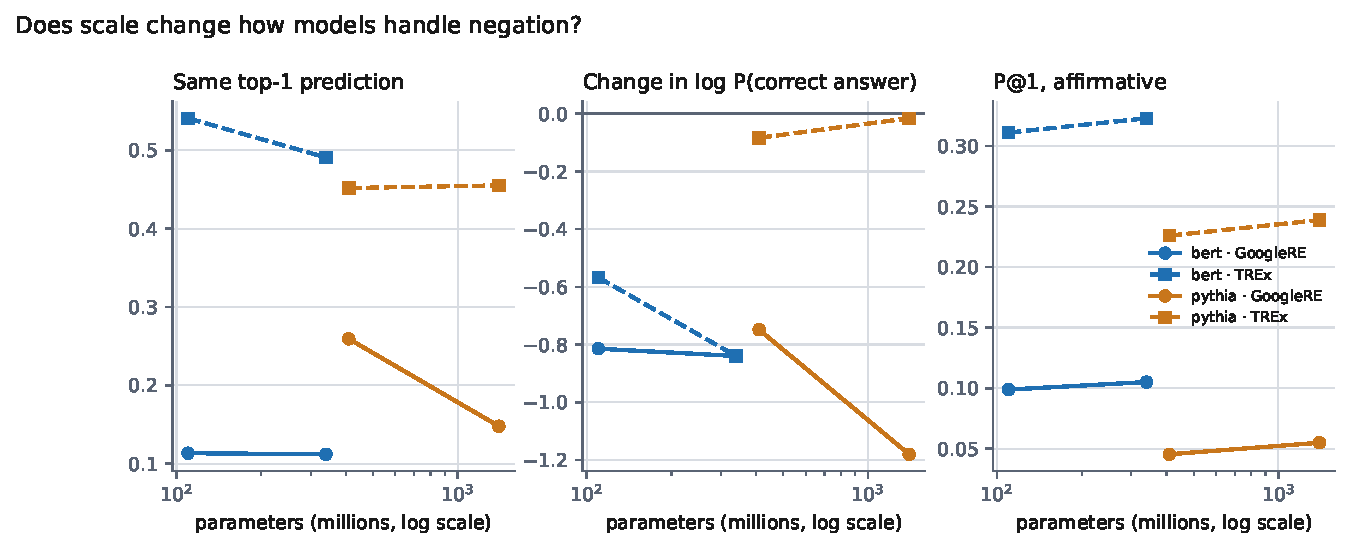
\includegraphics[width=\textwidth]{fig2_scaling.pdf}
\caption{Metrics plotted against parameter count (log scale), organised by model family and subset. Factual accuracy (right) improves with model size in both families, but the negation metrics (left, centre) show inconsistent gains, and for Pythia on T-REx $\Delta$ moves towards zero. Item sets as in Figure~\ref{fig:models}; P@1 as defined in Section~\ref{sec:method}.}
\label{fig:scaling}
\end{figure}

\subsection{RQ4: truth judgements}
\label{sec:results-truth}

Table~\ref{tab:truth} reports Experiment C. On T-REx the instruction-tuned model judges
negated statements correctly in 62.2\,\% of cases --- clearly above the 50\,\% chance level --- while remaining 15.1 points below its accuracy on affirmative
statements. Pair consistency is 0.601, so for about two fifths of statement pairs the model returns the same
verdict for a statement and its negation. Limiting the analysis to facts whose affirmative statement the model judges correctly leaves the negated accuracy nearly unchanged at 0.660, indicating that the gap does not result from absent knowledge.

\begin{table}[t]
\centering\small
\caption{Experiment C, Qwen2.5-1.5B (base, four-example prompt) and Qwen2.5-1.5B-Instruct (chat template). Because the design is balanced, chance performance is 0.5, and a model without bias would answer ``True'' half the time.}
\label{tab:truth}
\begin{tabular}{llrrrrrr}
\toprule
Model & Data & Items & Acc.\ affirm. & Acc.\ neg. & Gap & Consistency & Says ``True'' \\
\midrule
Base     & Google-RE & 600     & 0.640 & 0.507 & 0.133 & 0.327 & 0.163 \\
Base     & T-REx     & 8{,}200 & 0.749 & 0.525 & 0.224 & 0.378 & 0.192 \\
Instruct & Google-RE & 600     & 0.653 & 0.567 & 0.087 & 0.433 & 0.257 \\
Instruct & T-REx     & 8{,}200 & 0.773 & 0.622 & 0.151 & 0.601 & 0.314 \\
\bottomrule
\end{tabular}
\end{table}



The aggregate hides how this accuracy arises, and the $2\times2$ design exists to reveal it. Table~\ref{tab:cells} presents the accuracy by cell.

\begin{table}[t]
\centering\small
\caption{Experiment C by cell. Each cell has 2{,}050 items on T-REx. The correct
answer is ``True'' only in the affirmative/gold and negated/distractor cells; for every model and subset, those are the two cells
where the model does worst.}
\label{tab:cells}
\begin{tabular}{llrrrr}
\toprule
 & & & \multicolumn{2}{c}{Instruct} & Base \\
Polarity & Object & Correct answer & T-REx & Google-RE & T-REx \\
\midrule
affirmative & gold       & True  & 0.690 & 0.460 & 0.569 \\
affirmative & distractor & False & 0.856 & 0.847 & 0.929 \\
negated     & gold       & False & 0.911 & 0.860 & 0.960 \\
negated     & distractor & True  & 0.332 & 0.273 & 0.089 \\
\bottomrule
\end{tabular}
\end{table}

The instruction-tuned model is strongly biased towards ``False'': on a balanced item set it answers ``True'' only 31.4\,\% of the time. The two cells where ``False'' is the right answer therefore score 0.856 and 0.911, and the two where ``True'' is correct only 0.690 and 0.332. In a balanced design such a bias cannot by itself lift accuracy above chance: a model that always picked ``False'' would get exactly 0.500 overall and the same on negated items. Qwen2.5-1.5B-Instruct achieves 0.697 overall and 0.622 on negated items, so the accuracy above chance must come from discrimination between true and false statements.

The discrimination is visible in the rate of ``True'' answers. In the affirmative cells the model answers ``True'' for 69.0\,\% of gold objects and 14.4\,\% of distractors, a margin of 55 points. For negated statements it answers ``True'' for 33.2\,\% of distractors, where the negated statement is true, and for 8.9\,\% of gold objects, a margin of 24 points in the correct direction; a model that ignored \emph{not} would show the affirmative margin reversed. The model therefore does register the negation, but the margin shrinks to less than half, and its negated accuracy of 0.622 is exactly 0.5 plus half of that 24-point margin. Because the model also answers ``True'' less often to negated statements (21\,\% against 42\,\%), part of that shrinkage reflects a shift in response bias rather than weaker discrimination; a bias-corrected sensitivity index ($d'$) falls from 1.56 to 0.91, to about three fifths. The pair consistency of 0.601 shows the same weakness from another angle: for about two fifths of statement pairs, adding \emph{not} does not alter the verdict.

\paragraph{Base versus instruction-tuned.} The base model, prompted with four fixed examples, knows the facts about as well: in the affirmative cells its margin in ``True'' answers is 50 points (56.9\,\% against 7.1\,\%) and its $d'$ is 1.64. Under negation that margin all but vanishes, to 5 points (8.9\,\% against 4.0\,\%, $d' = 0.41$), and its negated accuracy of 0.525 is close to chance; its pair consistency is 0.378. The same facts that the instruction-tuned model handles partly under negation are handled hardly at all by the model it was derived from. The two models are prompted differently (chat template against four examples), so this comparison cannot separate the effect of post-training from that of the prompt.

This bias towards denial mirrors the tendency \citet{chen2023} report for generation, where models generate sentences grounded in positive commonsense knowledge far more accurately than in negative knowledge. That opposite biases appear under different task formats is consistent with treating the bias as a property of the decision rule rather than of the stored knowledge, although the two studies use different models.

\begin{figure}[t]
\centering
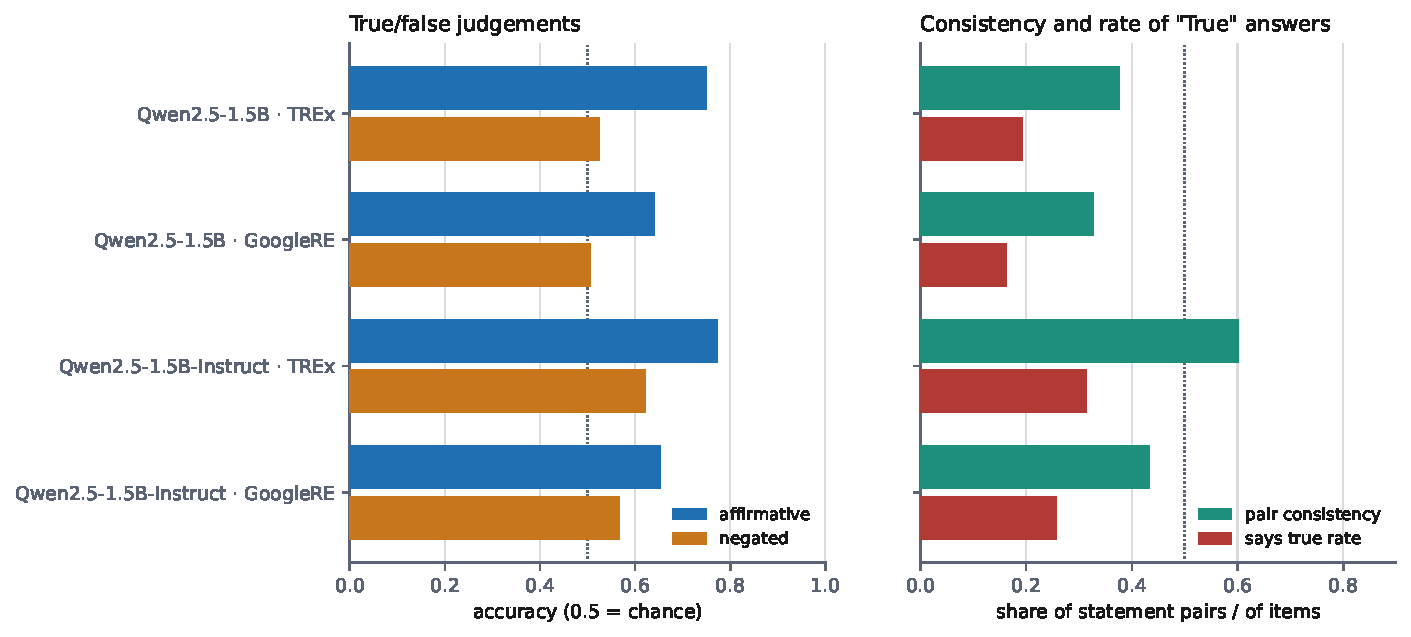
\includegraphics[width=0.85\textwidth]{fig4_truth.pdf}
\caption{Truth judgements for Qwen2.5-1.5B (base) and Qwen2.5-1.5B-Instruct. Left: accuracy by polarity for each model and subset, against the 0.5 chance
line. Right: pair consistency and the rate of ``True'' answers on a balanced item set.}
\label{fig:truth}
\end{figure}



\section{Reproducibility}
\label{sec:repro}

All code, per-model summaries, figures and the LaTeX source are in the repository
\url{https://github.com/PriyadithGowda/negprobe}. The repository documents each experiment and the command behind every table, and records the precision trap described in Section~\ref{sec:method}. It also commits the item-level outputs of every run reported here, including the BERT runs with the released templates, and a script that checks every result number in this paper against them. The cloze experiments involve no sampling, and the truth-judgement items are drawn with a fixed seed.

\section{Discussion}
\label{sec:discussion}

\paragraph{Each probe can mislead.} The same facts yield different verdicts under
different probes. The negated cloze query is a degenerate
task: it has no unique correct answer, so its metrics penalise a behaviour that is not clearly wrong,
and the strong reading of \citet{kassner2020} --- that models are insensitive to negation as such ---
is partly an artefact of that. The truth-judgement probe is protected against response bias in aggregate, because its design is balanced, but its cells are not: read on its own, the 0.911 on false negated statements would overstate the model's handling of negation, and the 0.332 on true ones would understate it. A probe for negation therefore needs either a balanced design reported cell by cell, as
here, or a measure anchored to the denied fact, as $\Delta$ is.

\paragraph{What $\Delta$ adds.} Because $\Delta$ is anchored to the denied fact rather than to the
ranking as a whole, it stays defined when no correct answer exists. It shows how much further BERT-large pushes the denied fact down on some relations, which overlap does not reveal, and for BERT against Pythia it reverses the ordering that overlap implies.
We would recommend reporting it alongside the original metrics in any future negation probe.

\paragraph{Implications for probing methodology.} Two incidents in this study point the same way. A
silent numerical failure produced a perfect-looking result, and a mislabelled template produced about a
fifth of an apparent effect. Both would have been invisible in a paper reporting only aggregate
scores. Probing results are cheap to produce and expensive to validate, which argues for publishing
per-relation numbers and item-level outputs as a matter of course.

\paragraph{Limitations.}
\label{sec:limitations}
(i) LAMA facts come from Wikipedia and are almost certainly included in the pretraining data of all models tested; while this does not affect the negation comparison, it means we cannot draw conclusions about knowledge acquisition. (ii) Each relation uses only one negation template, so the effects of template and negation are not separated; checking with paraphrases (such as \emph{never} or sentential negation) should be the next step. (iii) Our scaling results cover two model families, each at two sizes; larger versions of Pythia and Qwen were not tested because of limited compute resources (a consumer laptop and a free-tier T4 with daily limits), so we make no claims about scaling laws. (iv) The truth-judgement
experiment covers one base/instruct pair, prompted differently (four examples against the chat template), so the effect of post-training is not separated from that of the prompt. (v) ConceptNet and SQuAD are excluded, since their negations are
sample-specific rather than template-generated. (vi) The Pythia and Qwen runs were made on a GPU and the BERT runs on a CPU, all in float32; last-digit differences across hardware are possible.

\section{Conclusion}
\label{sec:conclusion}

We replicated the negated LAMA result for BERT and showed that a probability-based measure of negation
sensitivity can rank models differently from the original metrics. An autoregressive model alters its predictions more readily under negation than masked models of similar or smaller size, while suppressing the denied fact less. An
instruction-tuned model probed by truth judgement does register negation, scoring above chance on negated statements, but it discriminates markedly less well than on affirmative statements (its gap in ``True'' answers between true and false statements falls from 55 to 24 points) and answers ``False'' far more often than ``True''; its base model, which knows the facts about as well, barely registers the negation at all. Scale did not help consistently: within the Pythia family the larger model knows more facts but suppresses the denied
one no more. We also identified and corrected an error in the released templates that inflates the measured
effect: it invented a large effect for one relation (P190) and exaggerated a genuine one for another (P103). The
failure \citet{kassner2020} identified is real; its size depends on how one asks.

\begin{thebibliography}{99}

\bibitem[Biderman et al.(2023)]{biderman2023}
Stella Biderman, Hailey Schoelkopf, Quentin Anthony, Herbie Bradley, Kyle O'Brien, Eric Hallahan,
Mohammad Aflah Khan, Shivanshu Purohit, USVSN Sai Prashanth, Edward Raff, Aviya Skowron, Lintang
Sutawika, and Oskar van der Wal.
Pythia: A suite for analyzing large language models across training and scaling.
In \emph{Proceedings of the 40th International Conference on Machine Learning (ICML)}, 2023.
arXiv:2304.01373. \url{https://proceedings.mlr.press/v202/biderman23a.html}

\bibitem[Chen et al.(2023)]{chen2023}
Jiangjie Chen, Wei Shi, Ziquan Fu, Sijie Cheng, Lei Li, and Yanghua Xiao.
Say what you mean! Large language models speak too positively about negative commonsense knowledge.
In \emph{Proceedings of ACL 2023}. DOI: 10.18653/v1/2023.acl-long.550.
\url{https://aclanthology.org/2023.acl-long.550/}

\bibitem[Devlin et al.(2019)]{devlin2019}
Jacob Devlin, Ming-Wei Chang, Kenton Lee, and Kristina Toutanova.
BERT: Pre-training of deep bidirectional transformers for language understanding.
In \emph{Proceedings of NAACL-HLT 2019, Volume 1 (Long and Short Papers)}, pages 4171--4186.
DOI: 10.18653/v1/N19-1423. \url{https://aclanthology.org/N19-1423/}

\bibitem[Elsahar et al.(2018)]{elsahar2018}
Hady Elsahar, Pavlos Vougiouklis, Arslen Remaci, Christophe Gravier, Jonathon Hare, Frederique Laforest,
and Elena Simperl.
T-REx: A large scale alignment of natural language with knowledge base triples.
In \emph{Proceedings of the Eleventh International Conference on Language Resources and Evaluation
(LREC 2018)}. \url{https://aclanthology.org/L18-1544/}

\bibitem[Ettinger(2020)]{ettinger2020}
Allyson Ettinger.
What BERT is not: Lessons from a new suite of psycholinguistic diagnostics for language models.
\emph{Transactions of the Association for Computational Linguistics}, 8:34--48, 2020.
DOI: 10.1162/tacl\_a\_00298. \url{https://aclanthology.org/2020.tacl-1.3/}

\bibitem[García-Ferrero et al.(2023)]{garciaferrero2023}
Iker García-Ferrero, Begoña Altuna, Javier Álvez, Itziar Gonzalez-Dios, and German Rigau.
This is not a dataset: A large negation benchmark to challenge large language models.
In \emph{Proceedings of EMNLP 2023}. arXiv:2310.15941.
\url{https://aclanthology.org/2023.emnlp-main.531/}

\bibitem[Hosseini et al.(2021)]{hosseini2021}
Arian Hosseini, Siva Reddy, Dzmitry Bahdanau, R. Devon Hjelm, Alessandro Sordoni, and Aaron Courville.
Understanding by understanding not: Modeling negation in language models.
In \emph{Proceedings of NAACL-HLT 2021}. arXiv:2105.03519.
\url{https://aclanthology.org/2021.naacl-main.102/}

\bibitem[Kassner and Schütze(2020)]{kassner2020}
Nora Kassner and Hinrich Schütze.
Negated and misprimed probes for pretrained language models: Birds can talk, but cannot fly.
In \emph{Proceedings of ACL 2020}, pages 7811--7818. DOI: 10.18653/v1/2020.acl-main.698.
\url{https://aclanthology.org/2020.acl-main.698/}

\bibitem[McKenzie et al.(2023)]{mckenzie2023}
Ian R. McKenzie, Alexander Lyzhov, Michael Pieler, Alicia Parrish, Aaron Mueller, Ameya Prabhu, Euan
McLean, Aaron Kirtland, Alexis Ross, Alisa Liu, Andrew Gritsevskiy, Daniel Wurgaft, Derik Kauffman,
Gabriel Recchia, Jiacheng Liu, Joe Cavanagh, Max Weiss, Sicong Huang, The Floating Droid, Tom Tseng,
Tomasz Korbak, Xudong Shen, Yuhui Zhang, Zhengping Zhou, Najoung Kim, Samuel R. Bowman, and Ethan
Perez.
Inverse scaling: When bigger isn't better.
arXiv:2306.09479, 2023. \url{https://arxiv.org/abs/2306.09479}

\bibitem[Paszke et al.(2019)]{paszke2019}
Adam Paszke, Sam Gross, Francisco Massa, Adam Lerer, James Bradbury, Gregory Chanan, Trevor Killeen,
Zeming Lin, Natalia Gimelshein, Luca Antiga, Alban Desmaison, Andreas Köpf, Edward Yang, Zach DeVito,
Martin Raison, Alykhan Tejani, Sasank Chilamkurthy, Benoit Steiner, Lu Fang, Junjie Bai, and Soumith
Chintala.
PyTorch: An imperative style, high-performance deep learning library.
In \emph{Advances in Neural Information Processing Systems 32 (NeurIPS 2019)}. arXiv:1912.01703.
\url{https://arxiv.org/abs/1912.01703}

\bibitem[Petroni et al.(2019)]{petroni2019}
Fabio Petroni, Tim Rocktäschel, Sebastian Riedel, Patrick Lewis, Anton Bakhtin, Yuxiang Wu, and
Alexander Miller.
Language models as knowledge bases?
In \emph{Proceedings of EMNLP-IJCNLP 2019}. DOI: 10.18653/v1/D19-1250.
\url{https://aclanthology.org/D19-1250/}

\bibitem[Qwen Team(2025)]{qwen2025}
Qwen Team.
Qwen2.5 technical report.
arXiv:2412.15115, 2025. \url{https://arxiv.org/abs/2412.15115}

\bibitem[Truong et al.(2023)]{truong2023}
Thinh Hung Truong, Timothy Baldwin, Karin Verspoor, and Trevor Cohn.
Language models are not naysayers: An analysis of language models on negation benchmarks.
In \emph{Proceedings of *SEM 2023}. arXiv:2306.08189.
\url{https://aclanthology.org/2023.starsem-1.10/}

\bibitem[Wolf et al.(2020)]{wolf2020}
Thomas Wolf, Lysandre Debut, Victor Sanh, Julien Chaumond, Clement Delangue, Anthony Moi, Pierric
Cistac, Tim Rault, Remi Louf, Morgan Funtowicz, Joe Davison, Sam Shleifer, Patrick von Platen, Clara
Ma, Yacine Jernite, Julien Plu, Canwen Xu, Teven Le Scao, Sylvain Gugger, Mariama Drame, Quentin
Lhoest, and Alexander Rush.
Transformers: State-of-the-art natural language processing.
In \emph{Proceedings of EMNLP 2020: System Demonstrations}, pages 38--45.
DOI: 10.18653/v1/2020.emnlp-demos.6. \url{https://aclanthology.org/2020.emnlp-demos.6/}

\end{thebibliography}

\appendix

\section{Contribution Summary}
\label{app:contribution}

This appendix states what is new here relative to the works cited.

\paragraph{Novel relative to \citet{kassner2020}.} That paper introduces the negated probes and the two
rank-based metrics. We add (i) the probability-based measure $\Delta$, which remains defined for a
query with no unique answer and which can rank models differently from the rank metrics; (ii) a comparison
of masked models with a modern autoregressive model family on an explicitly matched item set (their study included Transformer-XL, but not a controlled scaling suite);
(iii) the truth-judgement probe, which tests whether their conclusion is format-dependent; and (iv) a
correction to their released templates.

\paragraph{Novel relative to \citet{truong2023} and \citet{garciaferrero2023}.} Both show that newer
models fail negation benchmarks. Neither applies the original negated LAMA probes while holding
templates and metrics fixed, so neither can attribute a difference to the model rather than the
benchmark. Our design holds the probe constant and varies architecture, scale and instruction tuning.

\paragraph{Reproducibility artefacts.} Code, configuration and per-item outputs are released at
\url{https://github.com/PriyadithGowda/negprobe}. Every figure in the paper is regenerated from those outputs by a single
script.

\section{Micro averages and additional tables}
\label{app:micro}

Main-text figures are macro averages (within relation, then across relations), following
\citet{petroni2019}. Micro averages over all pairs differ; for BERT-large on T-REx, overlap is
0.491 macro and 0.479 micro, with repaired templates. The full per-model micro and macro
figures are in \texttt{results/*/summary.csv} and the per-relation table in
\texttt{figures/table2\_relations.csv} of the repository.

\begin{table}[h]
\centering\small
\caption{Macro versus micro averages, T-REx, repaired templates.}
\begin{tabular}{lrrrrrr}
\toprule
& \multicolumn{2}{c}{$\rho$} & \multicolumn{2}{c}{Overlap} & \multicolumn{2}{c}{$\Delta$} \\
Model & macro & micro & macro & micro & macro & micro \\
\midrule
BERT-base  & 0.887 & 0.883 & 0.541 & 0.525 & $-0.568$ & $-0.590$ \\
BERT-large & 0.852 & 0.849 & 0.491 & 0.479 & $-0.840$ & $-0.906$ \\
\bottomrule
\end{tabular}
\end{table}

\section{Use of Generative AI}
\label{app:ai}

\paragraph{Tool.} Claude (Anthropic), a generative AI model, used through the Claude desktop
application in September 2026 as an assistant for programming, analysis and drafting.

\paragraph{Research design and decisions.} I chose the topic and the study to replicate
\citep{kassner2020}. The research questions were developed by me in dialogue with the AI. I decided
which models to compare within the compute available to me, which experiments to run, and how to
handle the error in the released templates, including re-running the affected models with corrected
templates and adding the base-model comparison. The AI proposed and discussed options; the decisions
were mine.

\paragraph{Code.} The \texttt{negprobe} package, the analysis, figure and verification scripts, and
the Colab notebook were implemented by the AI to my specifications. I ran every experiment myself, on my
own computer and on Google Colab, and reviewed the code and its outputs.

\paragraph{Data and analysis.} All model outputs were produced by those runs. Aggregate statistics,
tables and figures were computed from them with AI assistance; every result number in this paper is checked against the released outputs by a verification script. The error in the released templates
(Section~\ref{sec:data-error}) was identified during AI-assisted analysis and confirmed by inspecting
the data file directly.

\paragraph{Text.} A first draft of this paper was generated by the AI. I revised it, rewrote
substantial passages in my own words, and decided on the final content. The interpretation of the
results was developed in dialogue with the AI and reflects my conclusions.

\paragraph{Literature.} Candidate references were located with AI-assisted web search. Every reference was checked against the publisher's page (ACL Anthology, PMLR, NeurIPS proceedings or arXiv) for authors, venue and year, and every statement about a cited work was checked against the work itself.

\paragraph{Extent.} The AI's assistance was substantial for the code and the first draft of the text.
The research design, the decisions on scope and method, and the final text are my responsibility,
including their correctness.

\end{document}
